\textcolor{blue}{Problem 4}

7.13 Erasures and errors in a binary channel. Consider a channel with
binary inputs that has both erasures and errors. Let the probability of error be $\epsilon$ and the probability of erasure be $\alpha$, so the channel is follows:

\begin{figure}[htbp]
    \centering
	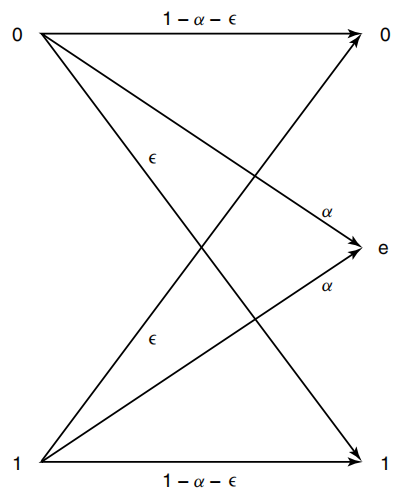
\includegraphics[width=0.3\textwidth]{../figures/7.13.png}
\end{figure}

(a) Find the capacity of this channel.

(b) Specialize to the case of the binary symmetric channel ($\alpha = 0$).

(c) Specialize to the case of the binary erasure channel ($\epsilon = 0$).

\textcolor{blue}{Solution}

(a) Let $p(X=0)=\pi, p(X=1)=1-\pi$, then we have
\begin{align*}
p(Y=0) &= \sum_{x}p(Y=0|X=x)p(X=x) = \pi(1-\alpha-2\epsilon) + \epsilon \\
p(Y=1) &= \sum_{x}p(Y=1|X=x)p(X=x) = \pi(2\epsilon+\alpha-1) + 1 - \alpha - \epsilon \\
P(Y=e) &= \alpha
\end{align*}
So we have
\begin{align*}
I(X;Y) &= H(Y) - H(Y|X) \\
&= H(Y) - \sum_{x}p(X=x)H(Y|X=x) \\
&= H\left(\alpha, \pi(1-\alpha-2\epsilon) + \epsilon, \pi(2\epsilon+\alpha-1) + 1 - \alpha - \epsilon\right) - H\left(1-\alpha-\epsilon,\alpha,\epsilon\right) \\
&= -\left[\pi(2\epsilon+\alpha-1) + 1 - \alpha - \epsilon\right]\log\left[\pi(2\epsilon+\alpha-1) + 1 - \alpha - \epsilon\right] - \left[\pi(1-\alpha-2\epsilon) + \epsilon\right]\log\left[\pi(1-\alpha-2\epsilon)+ \epsilon\right] \\
&\quad  + \epsilon\log\epsilon + \left(1-\alpha-\epsilon\right)\log\left(1-\alpha-\epsilon\right) \\
&\triangleq f(\pi) \\
f'(\pi) &= -\left(2\epsilon+\alpha-1\right)\log\left[\pi(2\epsilon+\alpha-1) + 1 - \alpha - \epsilon\right] - \left(1-\alpha-2\epsilon\right)\log\left[\pi(1-\alpha-2\epsilon)+ \epsilon\right] \\
f''(\pi) &= -\left(2\epsilon+\alpha-1\right)^2\log_e2\left[\dfrac{1}{\pi(2\epsilon+\alpha-1) + 1 - \alpha - \epsilon}+\dfrac{1}{\pi(1-\alpha-2\epsilon) + \epsilon}\right]
\end{align*}
Then we need to discuss the sign of $2\epsilon+\alpha-1$ to determine the sign of $f''(\pi)$. Since $\pi\in[0,1]$, so: \\
1. If $2\epsilon+\alpha-1=0$, then $f''(\pi)=0$. \\
2. If $2\epsilon+\alpha-1>0$, then
\begin{align*}
\left[\pi(2\epsilon+\alpha-1) + 1 - \alpha - \epsilon\right]_{\min} &= \left[\pi(2\epsilon+\alpha-1) + 1 - \alpha - \epsilon\right]\bigg|_{\pi=0} = 1-\alpha-\epsilon\geq 0 \\
\left[\pi(1-\alpha-2\epsilon) + \epsilon\right]_{\min} &= \left[\pi(1-\alpha-2\epsilon) + \epsilon\right]\bigg|_{\pi=1} = 1 - \alpha - \epsilon\geq 0
\end{align*}
So $f''(\pi)\leq 0$. \\
3. If $2\epsilon+\alpha-1<0$, then
\begin{align*}
\left[\pi(2\epsilon+\alpha-1) + 1 - \alpha - \epsilon\right]_{\min} &= \left[\pi(2\epsilon+\alpha-1) + 1 - \alpha - \epsilon\right]\bigg|_{\pi=1} = \epsilon\geq 0 \\
\left[\pi(1-\alpha-2\epsilon) + \epsilon\right]_{\min} &= \left[\pi(1-\alpha-2\epsilon) + \epsilon\right]\bigg|_{\pi=0} = \epsilon\geq 0
\end{align*}
So $f''(\pi)\leq 0$. \\

So above all, we have proved that $f''(\pi)\leq 0$ always holds, so $f(\pi)$ is concave.

In order to get that maximum value of $f(\pi)$, we have
$$f'(\pi^*)=0 \Rightarrow \pi^*=\dfrac{1}{2}$$
Then we have
$$C=\max_{p(x)}I(X;Y)=f(\pi^*)=H\left(\alpha,\dfrac{1-\alpha}{2},\dfrac{1-\alpha}{2}\right)-H(1-\alpha-\epsilon,\alpha,\epsilon)$$
And since we have
$$H\left(\alpha,\dfrac{1-\alpha}{2},\dfrac{1-\alpha}{2}\right)=-\alpha\log\alpha - 2 * \dfrac{1-\alpha}{2}\log\dfrac{1-\alpha}{2} = -\alpha\log\alpha - (1-\alpha)\log(1-\alpha)+1-\alpha=H(\alpha,1-\alpha)+1-\alpha$$

So above all, when $p(x)=\left(\dfrac{1}{2},\dfrac{1}{2}\right)$, the inequality takes the equality, i.e.
$$C=H(\alpha,1-\alpha)-H(1-\alpha-\epsilon,\alpha,\epsilon)+1-\alpha$$

(b) When $\alpha=0$, $C=1-H(\epsilon,1-\epsilon)$.

(c) When $\epsilon=0$, $C=1-\alpha$

\newpage